\documentclass{article}

\usepackage{microtype}
%\usepackage[english]{babel}
\usepackage{natbib}
\usepackage{amsmath}
\usepackage{graphicx}
\usepackage{hyperref}
\usepackage{float}
\usepackage{booktabs}
\usepackage{placeins}
\usepackage{subcaption}
\usepackage [autostyle, english = american]{csquotes}
\MakeOuterQuote{"}
\newcommand{\theHalgorithm}{\arabic{algorithm}}
\usepackage[accepted]{icml2021}
\usepackage{longtable}

\DeclareMathOperator*{\argmax}{argmax}
\DeclareMathOperator*{\argmin}{argmin}

\newcommand\numberthis{\addtocounter{equation}{1}\tag{\theequation}}

\icmltitlerunning{Heart Failure Prediction}

\begin{document}

\twocolumn[
\icmltitle{Heart Failure Prediction}

\icmlsetsymbol{equal}{*}

\begin{icmlauthorlist}
    \icmlauthor{Corey D. Cooke}{utk}
    \icmlauthor{Harshvardhan}{utk}
    \icmlauthor{Pragya Kandel}{utk}
    \icmlauthor{Vanessa Lama}{utk}
\end{icmlauthorlist}

%\icmlkeywords{Machine Learning, ICML}
\icmlaffiliation{utk}{University of Tennessee, Knoxville}

\icmlcorrespondingauthor{Corey D. Cooke}{ccooke7@vols.utk.edu}

\vskip 0.3in
]

\printAffiliationsAndNotice{}

\begin{abstract}

    Heart failure affects around 26 million people worldwide, according to \citet{cdc2021heartfailure}. The project aims to work on a dataset of 299 patients to predict heart failure and validate the prediction model based on several characteristics available with through the dataset. We will implement various stages of machine learning techniques such as feature selection and classification to develop this predictive model.

\end{abstract}

%---- First Report: Literature Review--------

\section{Introduction}

Heart failure is defined as a clinical condition when the heart is unable to pump enough blood and oxygen to support other organs in the body \citep{cdc2021heartfailure}. It affects around 26 million people worldwide making it a global pandemic \citep{savarese2017global}. In United States alone, 6.2 million adults suffer from heart failure and was the cause of 3,39,800 deaths in 2018 \citep{savarese2017global}. This situation is likely going to get worse and is predicted to affect 8 million people by 2030 \citep{lam2011epidemiology}. Heart failure not only affects the health of people but also impacts the economy of the country (United States of America). In 2012, when there were 5.7 million people with heart failure, it cost the nation an estimated 30.7 billion dollars, which was about 10 percent of total health expenditure \citep{cdc2021heartfailure}. The cost is estimated to increase by 128 percent between 2012 and 2030. 

Despite heart failure prevention being one of the top priorities for physicians, the forecasting of heart failure related events has not reached a high accuracy \citep{al2019clinical, dunn2007serum}. With the current advances in computing systems, machine learning can be an effective tool for predicting the survival of patients with heart failure symptoms and for the detection of risk factors that can indicate impending heart failure \citep{dunn2007serum}. With the available data on electronic heath records, machine learning can be used in understanding the patterns and correlations amongst a patient’s data \citep{awan2019machine}. This will give insight on the causes, severity, and understanding of the risk factors.

In this project, we would like to study the given data in the light of various machine learning tools. As part of our course, we were introduced to theory behind and practical implementation of feature selection, pre-processing of dataset, classification, neural networks, and support vector machines. The goal of this project is to use the theory and tools we've learned from the course to implement heart failure prediction and compare the performance of our model with respect to existing models and their performances. We will use performance metrics such as accuracy, run time, and confusion matrices to interpret our validation results.

\section{Dataset Details}

The dataset that will be extracted and used for the project is a reduced version of the complete dataset which was collected between April and December of 2015. There are 299 patients in the study. The information from patients were collected at the Faisalabad Institute of Cardiology and Allied Hospital in Faisalabad, located in the Punjab province of Pakistan. The dataset contains 13 features reporting on bodily, clinical, and lifestyle information about the patients. Some features such as anaemia, past instance of high blood pressure, diabetes, patient's sex, and smoking habits are binary in nature, while the rest are continuous. (For more details on dataset features see \citet{chicco2020machine}.) 

The dataset was originally used in a study by \citet{ahmad2017survival} and was later reused by \citet{chicco2020machine}, which is the paper cited on Kaggle, the site hosting this dataset \footnote{Larxel. (2019). Heart Failure Prediction: 12 Clinical Features For Predicting Death Events. \textit{Kaggle.} Accessed at \href{https://www.kaggle.com/andrewmvd/heart-failure-clinical-data}{https://www.kaggle.com/andrewmvd/heart-failure-clinical-data} on November 11, 2021.}.

\section{Survey of Previous Works}

\citet{ahmad2017survival} used various factors contributing to heart failure such as age, ejection fraction, anemia, and blood pressure  to predict mortality using the Cox regression. The result was further validated by computing calibration slope and discrimination ability via bootstrapping and found that age, renal dysfunction, blood pressure, ejection factor, and anemia significantly affected mortality. The prediction of survival of patients with heart failure of various features contributing to heart failure was done using various machine learning approaches such as linear regression, tree-based approach, artificial neural network (ANN), support vector machine (SVM), k-nearest neighbors (kNN) and Na\"ive Bayes (NB). 

The use of machine learning tools predicted that the two features of serum creatinine level and ejection fraction were enough to predict the survival of heart failure patients. It predicted the survival with higher accuracy than the use of original dataset \citep{chicco2020machine}.

In addition to studies on various factors contributing to heart failure, there have also been studies to compare the various machine learning algorithm on prediction of heart failure. The study by \citet{gurfidan2021classification} compared various machine learning algorithms for classification of death related to heart failure. They found that classification accuracy was highest with SVM (0.83) and lowest in kNN and decision tree classification (0.73). 

\citet{blecker2016comparison} compared heart failure identification using electronic health record data through different types of algorithms.
The first one, heart failure on problem list, second, presence of 1-2 characteristics, third logistic regression of 30 clinically relevant structured data elements, fourth, machine learning approach using unstructured notes and lastly, machine learning approach using structured and unstructured data. Upon analysis, they found that the area under ROC was highest in fifth approach (0.974) and lowest in third approach (0.953). While comparison of positive prediction value it was highest in the first algorithm (0.96) and lowest in the third approach (0.68).



\citet{awan2019feature} used the 47 features available in this dataset to predict the situation and outcomes of the patients. Building on their past study \citep{awan2019machine} that explored the ability of machine learning models to predict heart failure re-admissions and deaths, they check the importance of different features in the study. The previous study was complex and simpler models with similar accuracies were possible \citep{awan2019feature}. Note that the outcome of interest is whether an individual was readmitted to hospital or died, i.e. a binary variable. 

\citet{awan2019feature} uses several methods to select the important features. Initially, they do Fisher's t-test \citep{fisher1992statistical} to determine which variables were powerful enough to distinguish between the possible outcomes. The variables that could distinguish were included in the study. Furthermore, they also used Chi-squared test \citep{pearson1900x} to determine the variables that had significant association with the outcome variable.

They also try several other feature-selection methods like sequential forward selection and sequential backward selection which selects variable that improves accuracy most and reduces accuracy least, respectively (see \citet{marcano2010feature} and \citet{papatheocharous2012feature} for details of the method). Finally, they used Principal Components Analysis \citep{wold1987principal} for selection of variables. Notably, they did not use Fisher's Linear Discriminant Analysis \citep{cohen2014applied} for the purpose. The highest accuracy achieved was by the use of following variables: age, type of index admission, visit to an allied health professional in the last 6 months, length of hospital stay, use of antineoplastic and immunomodulating agents in the last 6 months, and history of HF, chronic kidney disease and depression \citep{awan2019feature}. It presented an AUC of 0.62 — same as the model which used all 47 variables.

%--- Insertion by Harsh ----------

\section{Technical Approaches}

In this section, we present a brief overview of ten different machine learning models used in this project.

\subsection{Maximum Posterior Probability Classifiers}

Maximum Posterior Probability (MPP) methods come from the set of statistical learning methods. The predicted class $\hat{\omega}$ is the one that maximizes the posterior probability, i.e.:

\begin{align*}
\hat{\omega} &= \underset{\omega_j}{\arg\max} \; P(\omega_j|x) \\
  &= \underset{\omega_j}{\arg\max} \; \frac{p(x|\omega_j)P(\omega_j)}{p(x)}, \numberthis \label{mpp}
\end{align*}

%\begin{gather}
%    \hat{\omega} = \underset{\omega_j}{\arg\max} \; P(\omega_j|x) \nonumber \\ 
%    = \underset{\omega_j}{\arg\max} \; \frac{p(x|\omega_j)P(\omega_j)}{p(x)}, \label{mpp}
%\end{gather}

where $p(x) = \sum_{i = 1}^c p(x|\omega_j)P(\omega_j)$. In general, it is assumed that the likelihood $p(x|\omega_j)$ is distributed normally with a mean $\boldsymbol\mu_j$ and covariance matrix $\boldsymbol\Sigma_j$. The choice of covariance structure decides the type of MPP classifier: Euclidean, Mahalanobis or Quadratic. The classification decision is made using the cost function, i.e. the observation belongs to the class which has the highest MPP.

\paragraph{Euclidean Classifier} In this classifier, the covariance for both classes is assumed to be:
\begin{equation}
    \boldsymbol\Sigma_1 = \boldsymbol\Sigma_2 = \sigma^2 \mathbf I
\end{equation}

This produces a linear decision boundary. For more details, see \citet{bishop2006pattern}.

\paragraph{Mahalanobis Classifier} In this classifier, the variance of the features is considered to be different from each other but considered same across classes. That is, if $\boldsymbol\Sigma_1$ is the sample covariance matrix computed from class 1 training samples and $\boldsymbol\Sigma_2$ is the sample covariance matrix computed from class 2 training samples, then the average of the two, i.e.
\begin{equation}
    \boldsymbol\Sigma = \frac{\boldsymbol\Sigma_1 + \boldsymbol\Sigma_2}{2} 
\end{equation}
is used for this classifier while calculating the MPP. For more details, see \citet{bishop2006pattern}.

\paragraph{Quadratic Classifier} In this classifier, $\boldsymbol\Sigma_1$ and  $\boldsymbol\Sigma_2$ are computed separately for each class and used in \eqref{mpp}. This results is a quadratic decision boundary.

\subsection{k-Nearest Neighbours}

The $k$-nearest neighbors (kNN) classifier chooses the test sample that is the closest to the majority vote among the $k$-nearest neighbors in Euclidean space. Ties are broken randomly.  To calculate the distance between points, Euclidean distance is used:

\begin{equation}
    d(x_1, x_2) = \sqrt{(x_1-x_2)'(x_1-x_2)}.
\end{equation}

Finally, the observation $x_i$ gets assigned to the class based on majority voting.

\begin{equation}
    P(Y = j|X = x)  = \frac{1}{K} \sum_{i \in A} I(y^{(i)} = j),
\end{equation}

where $I(.)$ is the binary indicator function giving value one when $y^{(i)} = j$ and zero otherwise.

For the implementation of kNN to our dataset, we used several values of k and tested the overall accuracy to pick the best k value for each dataset variation (nX, fX, pX). We can see this comparison in the the figures \ref{fig:kvalues}

\begin{figure}[h]
\begin{subfigure}{.4\columnwidth}
  \centering
  % include first image
  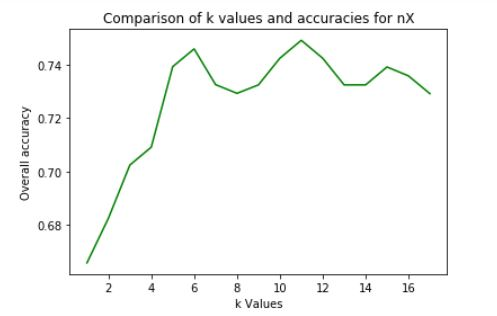
\includegraphics[width=\linewidth]{k_comparison_nX.JPG}  
  \caption{k for nX}
\end{subfigure} \hfill
\begin{subfigure}{.4\columnwidth}
  \centering
  % include second image
  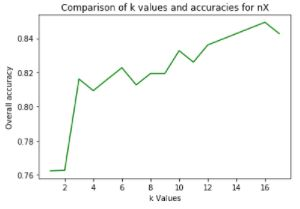
\includegraphics[width=\linewidth]{k_comparison_fX.JPG}  
  \caption{k for fX}
\end{subfigure} \hfill
\begin{subfigure}{.4\columnwidth}
  \centering
  % include second image
  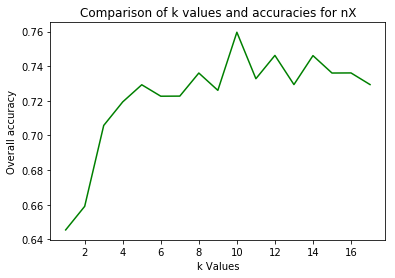
\includegraphics[width=\linewidth]{k_comparison_pX.png}  
  \caption{k for pX}
\end{subfigure} \hfill

\caption{Comparison of k values for kNN classifier.}
\label{fig:kvalues}
\end{figure}


\subsection{Back-propagation Neural Networks}

Back-propagation neural networks (BPNN), for the purposes of this document, can be described by a composition of affine functions with a sigmoid activation function. The sigmoid function $\sigma(x)$ is given by:
\begin{equation}
    \sigma(x) = \frac{1}{1 + e^{-x}}.
\end{equation}
If the scalar argument $x$ is replaced by a vector argument $\mathbf x$, the sigmoid is applied component-wise. We can define a single layer $i$ of the neural network as:
\begin{equation}
    f_i(\mathbf x) = \sigma ( \mathbf W_i \mathbf x + \mathbf b_i)
\end{equation}
where $\mathbf W_i$ is a weight matrix and $\mathbf b_i$ is a bias vector. The total neural network output $\mathbf y$ is given by the composition:
\begin{equation}
    \mathbf y = f_L(f_{L-1}( \ldots (f_2(f_1(\mathbf x) )) \ldots ))
\end{equation}
where the inner $L-1$ layers are referred to as ``hidden layers'' \citep{goodfellow2016deep}.  Training is performed by using gradient descent and recursively propagating derivatives back to the input layer, hence the name. 

\subsection{Support Vector Machines}

Support vector machines (SVM) are the combination of a linear method with a kernel trick applied to the input to increase the dimensionality of the feature space. The objective function to be maximized is the margin between the support vectors. Quadratic programming (QP) is used to solve this optimization problem \citep{bishop2006pattern}. For more details on the method, see \citet{noble2006support}.


\subsection{Random Forest}

The random forest (RF) method is a combination of a decision tree with bootstrap aggregation (``bagging'').  A ``forest'' of trees are trained using bagging as a training and fusing method. The general idea of a bagging method is that a combination of learning models will increase the overall result. A major advantage of random forest method is that it works for both classification and regression problems.

The algorithms was originally designed by \citet{breiman1996bagging}. In the original version, $a_n$ observations are drawn at random from the original dataset. Then, a tree-based model is built using these data points. At each node, a split is performed so as to maximise CART-criterion, or the cost function. The process is repeated several times with different set of data points. Finally, all such trees are merged together to form random forest. For more details on the method, see \citet{biau2016random}.

\subsection{Orthogonal Matching Pursuit}

The orthogonal matching pursuit (OMP) method  uses least squares to find the optimum linear model subject to a sparsity constraint (number of nonzero coefficients) \citet{sklearnlinear}. 

\subsection{Ridge Regression}

Ridge regression is a penalised least square method that uses an $L_2$ norm as a regularisation parameter. It penalises for model complexity and thus performs an indirect variable selection. The method forces coefficients of terms that least improve over a simple linear model to be close to zero, but not exactly equal to zero. For more details on the method, see \citet{eslr}.

\subsection{Logistic Regression}

Logistic regression is a linear model which has uses log odds of an event as the response. A common transformation to convert the class labels into posterior probabilities is called \textit{logit} transformation. 

\begin{equation}
    P(\omega_i|X = x) = \frac{\exp(\beta_0 + \beta'x)}{1+\exp(\beta_0+\beta'x)}.
\end{equation}

The decision boundary is constructed using the set of points for which the \textit{log-odds} are zero. This hyperplane is defined as the set $\{x: \beta_0 + \beta'x = 0\}$. For more details, see \citet{eslr}.

\subsection{Passive Aggressive Classifier}

The passive aggressive classifier is a linear model that is similar to the perceptron, but with the inclusion of a regularization parameter. Training is performed in a online method (one sample at a time); if the model output is correct, then no adjustments are made (``passive''), otherwise an adjustment is made (``aggressive''). See  \citet{crammer2006online} and \citet{sklearnlinear} for more details.

\subsection{Fusion Techniques}
We also implemented fusion using two classifiers, the squared Mahalanobis Distance classifier and the Quadratic Classifier (cases 2 and case 3 from our machine learning course. Then, we performed two Bayesian-based approach to fusion, Naive Bayes combination and Behavior-knowledge space (BKS).

%----- Second Report -----------------


\section{Exploratory Data Analysis}

Before jumping to feature selection and classification, we deemed it appropriate to visualize the dataset to get some idea of how it works. A bar plot showing patient outcomes is shown in Figure~\ref{fig:outcomeEDA}. It can be seen that approximately one-third of the patients in our dataset died of heart failure (class 1). A histogram of each feature is shown in Figure~\ref{fig:featuresEDA}.

It is noteworthy that some features are distributed in normally while some others have a bimodal distribution. Some features are presented as binary variables. Many statistical methodologies assume that the input dataset is distributed normally and thus we need to be cognisance of this potential violation. 

\begin{figure}[h]
    \centering
    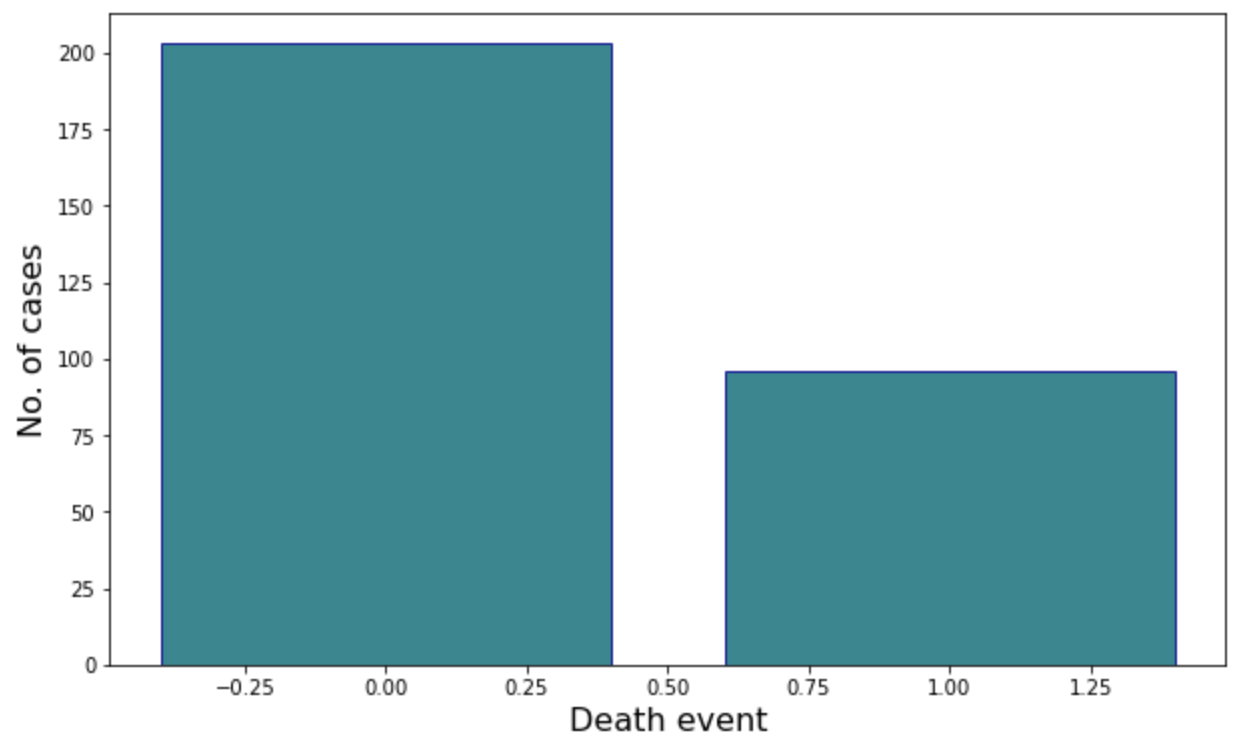
\includegraphics[width=0.55\linewidth]{outcomeEDA.png}
    \caption{Barplot showing patient outcomes. 1 represents death and 0 represents survival.}
    \label{fig:outcomeEDA}
\end{figure}

\begin{figure}[h]
    \centering
    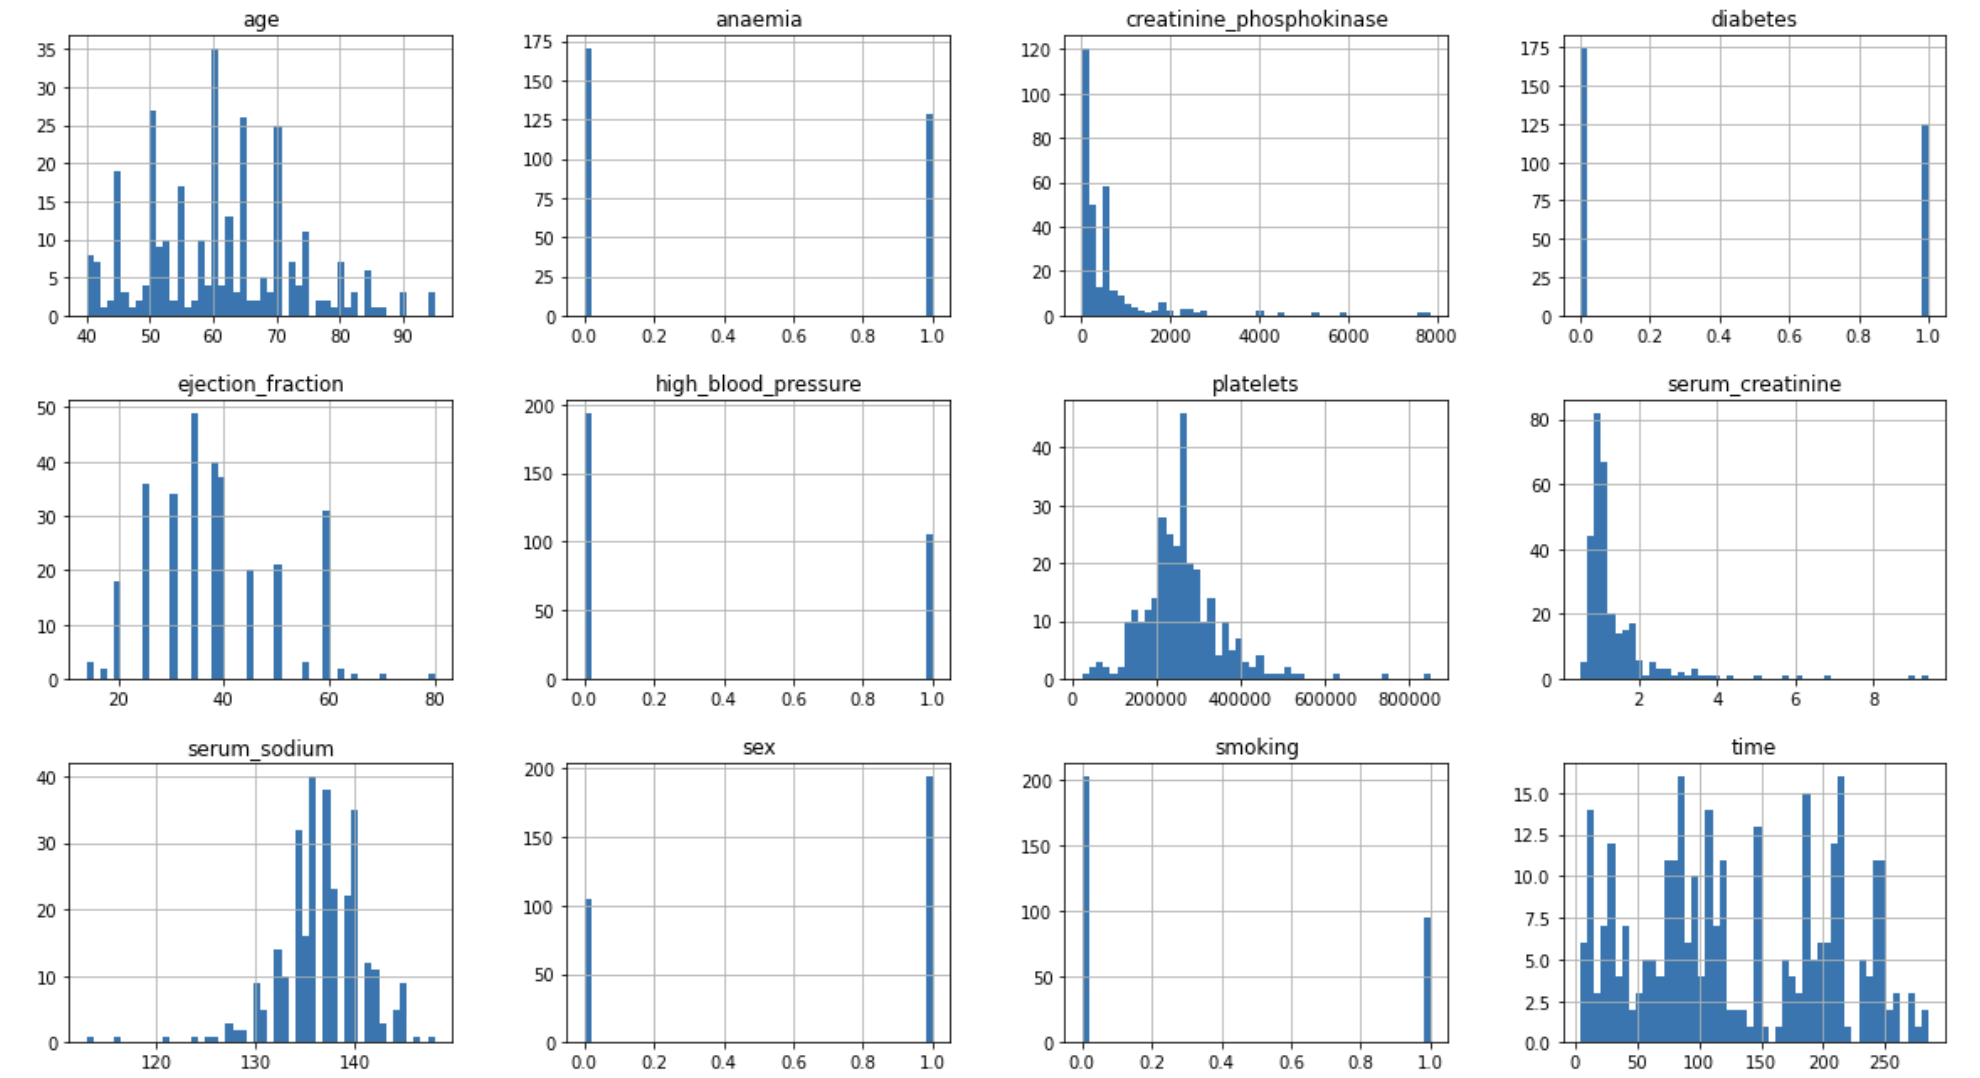
\includegraphics[width=0.98\linewidth]{featuresEDA.png}
    \caption{Histogram of 12 features present in the dataset. These 12 features are used to determine patient outcomes.}
    \label{fig:featuresEDA}
\end{figure}

\section{Machine Learning Pipeline}

In this project, we are trying are implementing a machine learning approach to predict heart failure from a selected set of clinical and biometric indicators. To perform this task, we will be applying the machine learning (ML) techniques which we learned in class. The data we have would be first preprocessed, followed by classification, and lastly, post-processing. The ML approach we will implement in this project is shown below in Figure~\ref{fig:mlpipe}.

\begin{figure}[h]
    \centering
    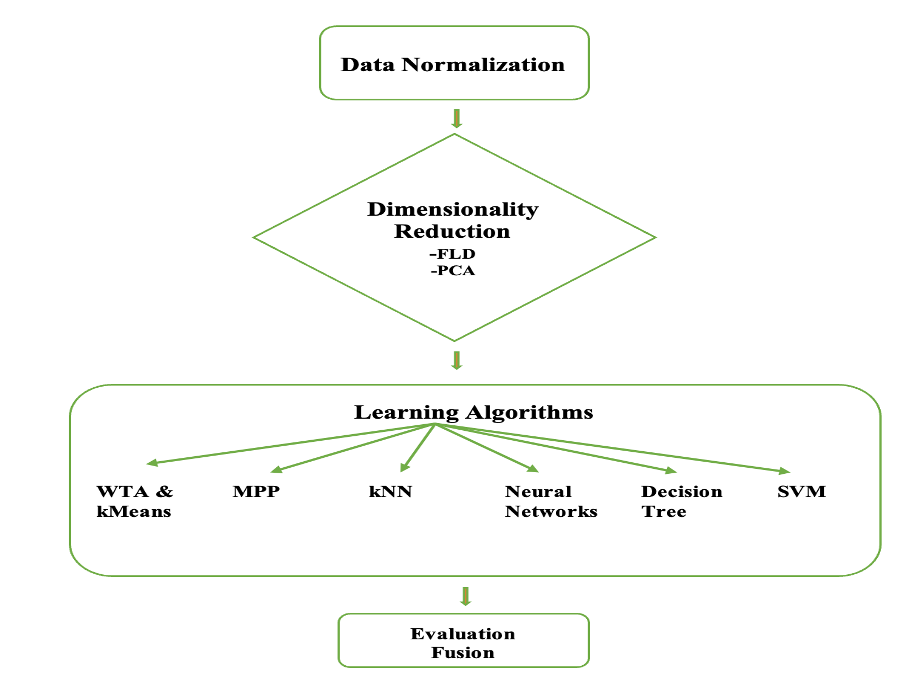
\includegraphics[width=0.6\linewidth]{Picture1.png}
    \caption{Schematic diagram the for machine learning pipeline of our project.}
    \label{fig:mlpipe}
\end{figure}

\paragraph{Design of Experiment} In a natural experiment or randomized clinical trial, we would conduct a factorial design for each input feature. Then, via experimentation we would conclude about each potential combination \citep{montgomery2017design}. 

Our design is quasi-experimental because we do not have a control group to compare against for effectiveness of our treatment variables. Our quasi-experimental design had 12 clinical features determining patient outcome. The goal is to determine patient outcome with the highest accuracy.

\section{Preprocessing of Data}

We are using the heart failure prediction data from Kaggle for this project. 
\footnote{Larxel. (2019). Heart Failure Prediction: 12 Clinical Features For Predicting Death Events. \textit{Kaggle.} Accessed at \href{https://www.kaggle.com/andrewmvd/heart-failure-clinical-data}{https://www.kaggle.com/andrewmvd/heart-failure-clinical-data} on November 11, 2021.}
The data has 13 categories and 299 samples. The information is divided into two classes based on death events: class 1 and class 0. 

In the first step, data would be standardized by subtracting the mean and dividing by standard deviation. We denote to this variation of our dataset as nX. Then, the standardized data is further pre-processed using the Fisher’s linear discriminant (FLD) method and principal component analysis (PCA) for dimensionality reduction as described later.

\paragraph{Dimensionality Reduction}

We applied the two dimensionality reduction methods on our raw data, which resulted in two more processed datasets as follows:
\begin{enumerate}
    \item FLD dataset, denoted as \texttt{fX},
    \item PCA dataset with $< 5\%$ error rate (i.e. keep $\geq 95\%$ of the variance), denoted as \texttt{pX}.
\end{enumerate}

In this report, we randomly split the data for validation using n-fold cross validation method with $n=5$.

\subsection{Overall Accuracies}

For the list of classifiers and fusion methods, we supplied them with the nX, fX, and pX datasets. Below is the list of all the overall accuracies. Tables \ref{tab:acccf1} to \ref{tab:acccf3} report the accuracies from different methods. These tables allows us to pick the highest overall accuracy for different types of pre-processed dataset applied to different classification and fusion approaches.

\begin{table}[h]
\centering
\begin{tabular}{@{}ll@{}}
\toprule
\multicolumn{2}{c}{Dataset with standardization (nX)}        \\ \midrule
Case 1                          & 0.79                  
\\
Case 2                          & 0.81                  \\
Case 3                          & 0.75                 \\
kNN (k = 6)                     & 0.74                  \\
BPNN                            & 0.90                  \\
SVM                             & 0.76                  \\
Random Forest                   & 0.78                 \\
Passive Aggressive Classifier   & 0.74                  \\
BKS (case 1 + case 2)           & 0.81                  \\
NB (case 1 + case 2)            & 0.83                  \\ \bottomrule
\end{tabular}
\caption{Overall accuracies for the nX dataset with classification and fusion approaches.}
\label{tab:acccf1}
\end{table}

\begin{table}[h]
\centering
\begin{tabular}{@{}ll@{}}
\toprule
\multicolumn{2}{c}{Dataset with FLD (fX)}                    \\ \midrule
Case 1                          & 0.82                  
\\
Case 2                          & 0.84                  \\
Case 3                          & 0.84                  \\
kNN (k = 13)                    & 0.83                  \\
BPNN                            & 0.83                  \\
SVM                             & 0.81                  \\
Random Forest                   & 0.85                  \\
Passive Aggressive Classifier   & 0.82                  \\
BKS (case 1 + case 2)           & 0.84                  \\
NB (case 1 + case 2)            & 0.84                  \\ \bottomrule
\end{tabular}
\caption{Overall accuracies for the fX dataset with classification and fusion approaches.}
\label{tab:acccf2}
\end{table}

\begin{table}[H]
\centering
\begin{tabular}{@{}ll@{}}
\toprule
\multicolumn{2}{l}{Dataset with PCA (pX)} \\ \midrule
Case 1                          & 0.83                  
\\
Case 2                          & 0.82                  \\
Case 3                          & 0.74                  \\
kNN (k = 10)                    & 0.75                  \\
BPNN                            & 0.83                  \\
SVM                             & 0.76                  \\
Random Forest                   & 0.69                  \\
Passive Aggressive Classifier   & 0.77                  \\
BKS (case 1 + case 2)           & 0.82                  \\
NB (case 1 + case 2)            & 0.83                  \\\bottomrule
\end{tabular}
\caption{Overall accuracies for the pX dataset with classification and fusion approaches.}
\label{tab:acccf3}
\end{table}

\section{Best Performance}

\paragraph{Confusion Matrices}
The confusion matrices are reported in Table \ref{tab:cfnx} to \ref{tab:cfpca}. The best performing classifiers were BPNN for nX dataset, Random Forest (only slightly) for the fX dataset, and BPNN and Naive Bayes fusion gave similar accuracies for pX dataset. Below are the confusion matrix for each case reflecting these outcomes.

\begin{table}[h]
\centering
\begin{tabular}{l|ll}
                & Predicted Positive & Predicted Negative \\ \hline
Actual Positive & 199                & 4                 \\
Actual Negative & 15                 & 81                
\end{tabular}
\caption{Confusion matrix for complete dataset with all features (nX).}
\label{tab:cfnx}
\end{table}

\begin{table}[h]
\centering
\begin{tabular}{l|ll}
                & Predicted Positive & Predicted Negative \\ \hline
Actual Positive & 188                & 15                 \\
Actual Negative & 28                 & 68                
\end{tabular}
\caption{Confusion matrix for data with features selected using FLD (fX).}
\label{tab:cffld}
\end{table}

\begin{table}[h]
\centering
\begin{tabular}{l|ll}
                & Predicted Positive & Predicted Negative \\ \hline
Actual Positive & 191                & 12                  \\
Actual Negative & 21                 & 75                
\end{tabular}
\caption{Confusion matrix for data with features selected using PCA w/ 5 percent error rate restriction (pX).}
\label{tab:cfpca}
\end{table}


\paragraph{ROC Curves}
The ROC curves is presented in Figure \ref{fig:grid1}. BPNN didn’t produce any ROC curve as it's hyper-parameter indirectly controlling the prior probability.

\begin{figure}[h]
\begin{subfigure}{.4\columnwidth}
  \centering
  % include first image
  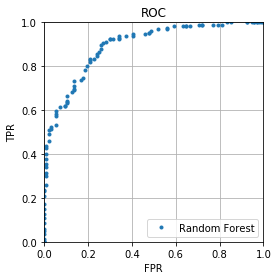
\includegraphics[width=\linewidth]{ROC_curve_fX.png}  
  \caption{fX with Random Forest}
\end{subfigure} \hfill
\begin{subfigure}{.4\columnwidth}
  \centering
  % include second image
  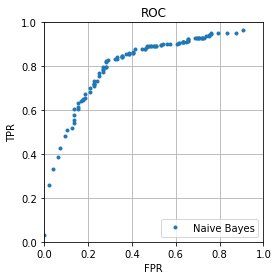
\includegraphics[width=\linewidth]{ROC_curve_pX_NB.png}  
  \caption{pX with Naive Bayes Fusion}
\end{subfigure} \hfill

\caption{ROC curves for best performance classification techniques for each variation of our dataset. BPNN didn’t produce any ROC curve as its hyper-parameter indirectly controls the prior probability.}
\label{fig:grid1}
\end{figure}


\paragraph{Comparison with Literature Review}

We also compared the results from our algorithm implementations with the implementations from different research papers. Accuracies for kNN, SVM and NB Fusion are taken from \citet{gurfidan2021classification}. Accuracies for BPNN, Random Forest and Passive-Aggressive classifier are taken from \citet{chicco2020machine}. The comparison is presented in Figure \ref{fig:comparison}. 

We could not find any literature that had implemented MPP classifiers or the BKS classifier on this data. Our best method, BPNN, performed significantly better than the state-of-the-art method. We tried finding the hyperparameters used by \citet{chicco2020machine} but due to incomplete information we couldn't replicate the same. We hypothesise that this drastic improvement is likely because of the choice of initial states for our model or theirs, choice of hyper-parameters, or a combination of both reasons.

\begin{figure}
    \centering
    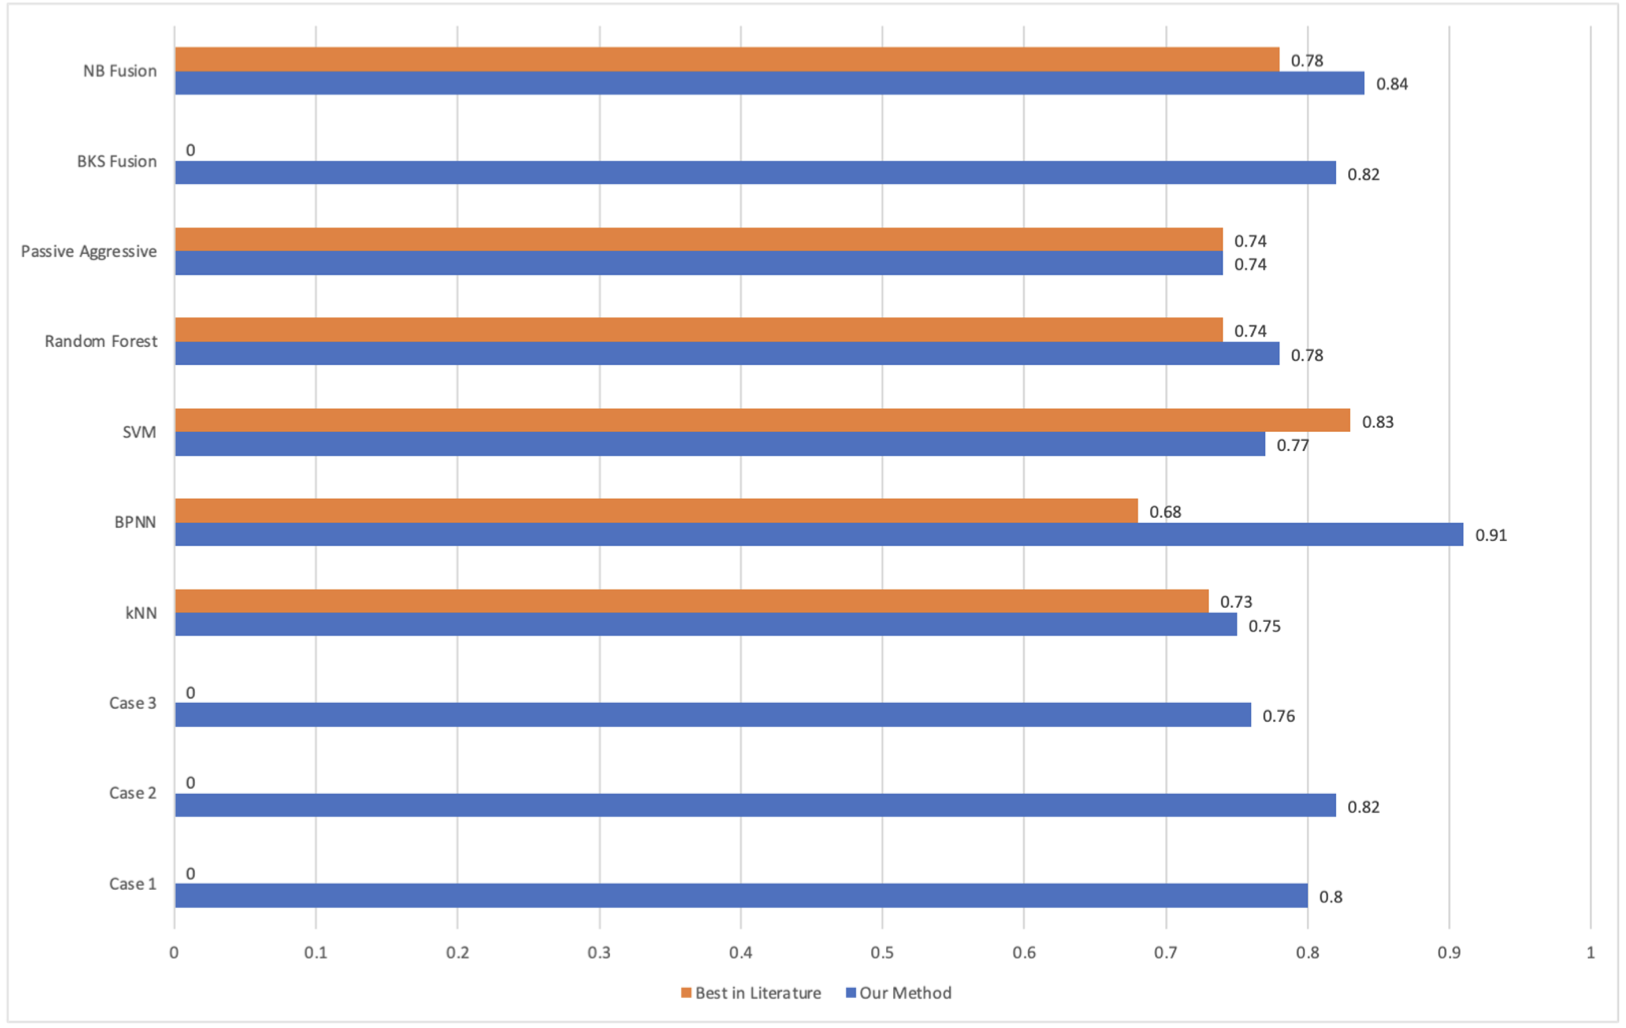
\includegraphics[width=\columnwidth]{comparison.png}
    \caption{Comparison with state-of-art implementation from literature review. Accuracies for kNN, SVM and NB Fusion are taken from \citet{gurfidan2021classification}. Accuracies for BPNN, Random Forest and Passive-Aggressive classifier are taken from \citet{chicco2020machine}. The comparison is presented in Figure \ref{fig:comparison}. }
    \label{fig:comparison}
\end{figure}

\section{Concluding Remarks}

Heart failure is a cause of concern in modern world. Our goal was to develop a machine to predict patient outcomes given other details. In our replication study we tried many classifiers on cardiac arrest and heart failure dataset. We found Back-propagation Neural Networks to be the best performing one with an accuracy of 91\%. 

The study is limited in its power. The data points we have are limited. Heart failure isn't a trivial issue and any model based on only 299 samples might lead to over-fit no matter what train/test/validate proportion we choose. Furthermore, the features are not well ascribed. It is unclear why certain features are treated as binary while others are continuous, even when the medical community would consider them continuous. There were a few past studies like \citet{awan2019feature} that considered manual non-algorithmic feature selection methods like t-test, Chi-squared test and F-test. These selection methods can be an extension to our project's current state. However, we didn't include it in our study as it was beyond the scope of this course and paper.

\citet{awan2019feature}

%\section{Discussion}
 
%Performance metrics for each of the method is presented in Tables \ref{tab:acccf1} to \ref{tab:acccf3}, using the prior probability estimated from the training data.  We can seen from this table and the prior section that FLD and the full 12-feature dataset perform nearly identically when using the Case 2 classifier.   This is not surprising, as they can be shown to be mathematically equivalent given perfect knowledge of the class covariance matrices. 


%Following this, we chose the most accurate input dataset and applied BKS and NB classifier fusion. Tables \ref{tab:acccf1} to \ref{tab:acccf3} report the accuracies obtained. Clearly, using fusion doesn't result in any drastic improvement.



\section*{Acknowledgement}

We present our sincere thanks to Prof Hairong Qi, Senjuti Dutta and Taher Naderi for their kind support and help throughout the course and this project.

\section*{Task Allocation}
The tentative task allocation between the group members has been described below. However, this was only considered as guide and not as a strict rule. All of us helped each other improve the team's contribution. This project wouldn't have been possible without extensive discussions between members on all aspects of the project.
\begin{itemize}
    \item Corey Cooke: Implementing classification and fusion methods; code review and re-usability; proof reading report drafts.
    \item Harshvardhan: Code review and implementation; performance evaluation and reporting; proof reading report drafts.
    \item Pragya Kandel: Code review and implementation; performance evaluation and reporting; proof reading report drafts.
    \item Vanessa Lama: Implementing validation and evaluation methods; code review and implementation; proof reading report drafts.
\end{itemize}

%\FloatBarrier
%\newpage

\bibliographystyle{icml2021}
\bibliography{references.bib}


\end{document}